\section{システムの概要}
本システムは，VR環境を活用し，仮想音源の音高（ピッチ）と空間的な位置関係を結びつけることで，聴覚と空間認識能力の向上を目指すVR学習支援アプリケーションである．学習の基盤として，12個の仮想音源（球体）を，視覚情報が集中する前方半円状に配置する「180度配置」と，全方位に配置する「360度配置」の2パターンを設定可能とし，学習目的に応じた柔軟なトレーニングを提供する．音源には，ピッチ識別が容易なピアノ音を採用しており\cite{pedersen2020spatialized}，これによりユーザは空間的な位置と特定のピッチとの対応関係を正確かつ効率的に習得することが期待される．
\section{使用機材}
本システムはヘッドマウントディスプレイ（HMD）により視覚，聴覚刺激を提示し，コントローラによる触覚刺激を利用する．HMDにはMeta Quest 2，コントローラにはMeta Quest 2のコントローラを用いた．また，アプリケーションの開発環境にはUnity 6を使用した．使用したHMDおよびコントローラを図\ref{fig:hardware}に示す．

\begin{figure}[H]\centering
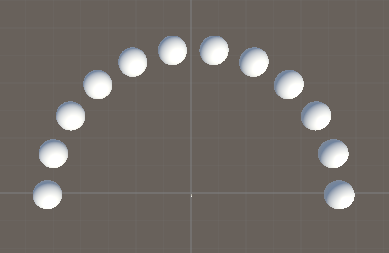
\includegraphics[width=100mm]{figure/system_hardware.png}\caption{実験で使用したHMDとコントローラ}\label{fig:system_hardware}
\end{figure}

\section{システムの設計実装}
\subsection{前方円状配置システム}\label{sec:system_180}
本研究で開発した「前方円状配置」システムの概要図を図\ref{fig:system_180_overview}に示す．

\begin{figure}[H]\centering
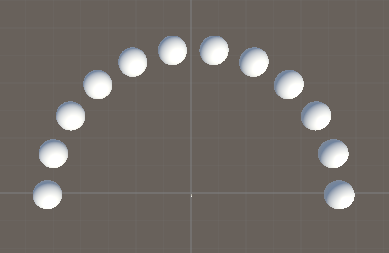
\includegraphics[width=100mm]{figure/system_180.png}\caption{180度配置}\label{fig:system_180_overview}
\end{figure}

180度配置の空間は，既存の音感トレーニングシステムを模した条件である．ユーザの前方を中心とした半円周上（水平角 $-90$度 $\sim$ $+90$度）に，12個の音源を等間隔に配置した．隣接する音源同士の角度間隔は約15度であり，音源密度が高い状態となっている．なお，音源の高さ（Y軸座標）については，一般的な鍵盤配置を想定し，全ての音源をユーザの耳の高さ（$Y=0$）で一定とした．

\subsection{全方位配置システム}\label{sec:system_360}
次に，本研究で提案する「全方位配置」システムの概要図を図\ref{fig:system_360_overview}および図\ref{fig:system_360_height}に示す．

\begin{figure}[H]\centering
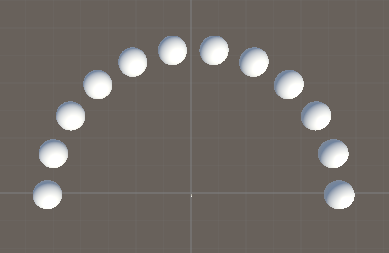
\includegraphics[width=100mm]{figure/system_360.png}\caption{上から見た360度配置}\label{fig:system_360_overview}
\end{figure}

\begin{figure}[H]\centering
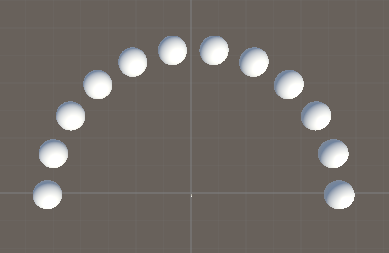
\includegraphics[width=100mm]{figure/system_360.png}\caption{横から見た360度配置}\label{fig:system_360_height}
\end{figure}

図3.3で示した全方位配置は，本研究で提案する全周囲を活用した条件である．基準音（C3）から1オクターブ上の音（B3）までの全12音（半音階）を配置対象とし，各音源オブジェクトはユーザを中心として等距離・等間隔に配置される．音源の高さ（Y軸座標）については，音高の上昇に伴って螺旋状に上昇する配置を採用した．この際，音源間の距離設定には音階ごとの周波数比を用い，以下の式を適用した．

\begin{equation}
    d = d_0 \times \frac{f}{f_0}\label{eq:dist_linear}
\end{equation}

ここで，$d$は中心から対象音源までの距離，$d_0$は中心から基準音までの距離，$f$は対象音源の周波数，$f_0$は基準音の周波数である．また，周波数は以下の式で平均律に基づく音名に割り当てることができる．

\begin{equation}
    f = f_0 \times (2)^{\frac{n}{12}} \label{eq:freq_linear}
\end{equation}

ここで，$n$は基準音からの半音数，$f$は基準音から$n$半音上の音の周波数，$f_0$は基準音の周波数である．この式に従い，周波数の物理的な変化（Hzの増加）をそのまま空間的な距離の比率として変換を行っている．

\subsection{システムの共通機能}
\ref{sec:system_180}および\ref{sec:system_360}で述べた2つのシステムに共通する機能について説明する．本システムにはPractice ModeとTest Modeの2つのモードが存在する．Training Modeでは，ユーザが任意の音源オブジェクトをコントローラで選択することで，対応する音高の音が再生される．これにより，ユーザは各音源の位置と音高の対応関係を自由に確認できる．一方，Test Modeでは，ピッチインターバルをTraining Modeで確認している音源の配置にしたがい，ユーザはその位置に対応する音源オブジェクトをコントローラで選択することで回答を行う．問題数は全部で24問あり，正解・不正解のフィードバックは選択した瞬間にUIとして表示されるように設計した，ユーザは自身の回答結果を後で確認できる．また，Test Modeでは各モード終了後に正答率が表示される．さらに，両モードともに，コントローラの振動機能を用いて触覚フィードバックを提供する．ユーザが音源オブジェクトに近づくと振動強度が増加し，遠ざかると減少する仕組みとなっている．
